Classical computer vision has limitations and is not near the performance of the human visual system. Processing high-resolution is still a challenge in terms of power and memory consumption for general purpose computers, even more if it's a mobile platform. Interpretation of what is sensed is another weak aspect of computer vision, while a computer may beat a human reading a license plate of a moving vehicle, it is sometimes necessary for a human to supervise the read-out. ANNs have recently been shown to produce some very  good results in the field of image recognition~\cite{krizhevsky2012imagenet}, but these models focus only on this task and do not account for the large number of feedback connections found in the brain.
%The use of ANN for image recognition has recently shown successful results~\cite{krizhevsky2012imagenet}. Unfortunately this is just one of the many functions of the visual system, to the best of our knowledge, most models of visual functions are based in a few parts of the visual cortex. For some tasks (e.g. image recognition), most models are using a feed-forward approach but that doesn't account for any of the back projections observed in the brain.

An observed characteristic in the visual system is the use of simple and complex cells, which are present in different layers along the visual cortex~\cite{hubel1962receptive,thompson2000brain}. The presence of these cells could explain the preferred activation of some neurons to bars in a certain orientation. Simple cells receive information from one or more neurons coming the retina and the LGN. Complex cells' inputs come from one or more simple cells, allowing them to respond to a particular orientation in a region of the retina. Figure~\ref{fig:vision:simple-complex} shows an example of the connectivity of simple and complex cells.

\begin{figure}[h]
  \begin{center}
    \begin{subfigure}[t]{0.4\textwidth}
      \includegraphics[width=\textwidth]{simple-complex-diag-bar}
      \caption{Response to a diagonal bar.}
    \end{subfigure}
    \begin{subfigure}[t]{0.4\textwidth}
      \includegraphics[width=\textwidth]{simple-complex-horiz-bar}
      \caption{Response to a horizontal bar.}
    \end{subfigure}
    \caption{Diagrams of the simple and complex cells (adapted from~\cite{wikipedia-images}). }
    \label{fig:vision:simple-complex}
  \end{center}
\end{figure}

Some models make use of hierarchical topologies that resemble the organization of the visual cortex. The main idea behind a hierarchy is that successive layers encode more complex patterns than the previous one. For example, Figure~\ref{fig:vision:hierarchical_encoding} shows a fictional network whose units in the first layer respond to oriented edges. The next layer has a preference for corners and, finally, the third layer responds better to shapes.

\begin{figure}[h]
  \begin{center}
    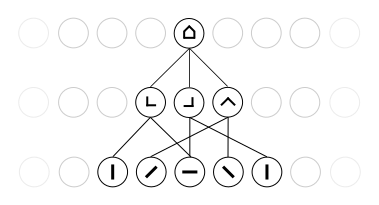
\includegraphics[width=0.5\textwidth]{hierarchical_encoding}
    \caption{Progressively more complex features in each successive layer.}
    \label{fig:vision:hierarchical_encoding}
  \end{center}
\end{figure}

The following are examples of hierarchical neural networks that also fall into the deep network category since they use more than one hidden layer.
The Neocognitron is an example of a hierarchical topology which uses the simple-complex cell concept~\cite{fukushima1988neocognitron}; simple cells from one layer sample from complex cells in the previous. The downside of this model is that it has been proven to be hard to train.

A variation of the simple-complex cell architecture is known as HMAX~\cite{riesenhuber1999hierarchical}. The simple cells perform template matching through a weighed sum of their input and the complex a softmax operation. The softmax operation selects the best candidate of the simple cells and transmits that to the next layer.

Yet another adaptation of the simple-complex architecture is used in Convolutional Networks~\cite{lecun-1990handwritten}. Here, complex cells perform a convolution of their inputs and simple cells sub-sample the output of complex cells.

Hierarchical networks have been shown to provide geometric transformation invariance, though most examples only model feed-forward connectivity. Recurrent networks are among the few that use feed-back in their design. Though they might be difficult to use due to unwanted interactions between layers. They have been used successfully for spatio-temporal pattern and hand-written text recognition, and motor control. A model known as \emph{LAMINART} makes use of feedback connections, and it's based the laminar circuits of the cortex~\cite{raizada2003laminart}. The model is biologically plausible and has been adapted to simulate different perceptual effects. The \emph{Neural Abstraction Pyramid} architecture is another model that is bio-inspired and uses lateral and feedback connections~\cite{behnke2003hierarchical}. It's been used for various visual tasks such as image recognition and face localization.

